% sample file for Modelica Conference paper

\documentclass[11pt,a4paper,twocolumn]{article}
\usepackage{graphicx}
\graphicspath{{fig/}}
\usepackage[T1]{fontenc}
\usepackage[british]{babel}      % some british specific settings
\usepackage[utf8]{inputenc}    %% european characters can be used
\usepackage{lmodern,amsmath,mathptmx,url}      %% recommended for readable pdf
\pagestyle{empty}                %% no page numbers!
\usepackage{geometry}            %% please don't change geometry settings!
\geometry{left=20mm, right=20mm, top=25.4mm, bottom=25mm, noheadfoot, columnsep=8mm}
\parindent0pt
\bibliographystyle{ieeetr}

% some additional packages
\usepackage{listings} % for code listings
\usepackage{color}

% usefull commands
\newcommand{\myr}{\textsuperscript{\textregistered}}
\newcommand{\ud}{\mathrm{d}}
\newcommand{\matx}[1]{\mathbf{#1}}
\newcommand{\impact}{\texttt{impact.py}}

\begin{document}

\title{\textbf{{\small Modelica'2014}\\
    \texttt{impact.py} -- A Modelica\myr\ Package Manager}}

\author{Michael Tiller\\Xogeny Inc., USA\\\url{michael.tiller@xogeny.com} %
        \and Dietmar Winkler\\Telemark University College, Norway\\\url{dietmar.winkler@hit.no}}
\date{} % <--- leave date empty
\maketitle\thispagestyle{empty} %% <-- you need this for the first page

\section*{Abstract}

To manage complexity, modern programming languages use organizational
units to group code related by some common purpose.  Depending on the
programming language, these units might be called libraries, packages
or modules.  But they all attempt to encapsulate functionality to
promote modular code and reusability.  For the remainder of this
paper, we will simply refer to these organizational units as
\em{packages} (as they are called in Modelica).

Also common to many modern programming languages are tools that can be
used to manage these packages.  These tools are generally called
\em{package managers} and they allow developers to quickly "fetch" any
packages they may need for a given project.  The main functions of
package managers are to allow developers to search, install, update
and uninstall packages with a simple command-line or graphical
interface.  In the Java world, the most common package manager is
\tt{maven}.  For Python, tools like \tt{easy_install} and \tt{pip} are
used for managing packages.  For client-side web development,
\tt{bower} is used.  For server-side javascript, the tool of choice is
\tt{npm}.  For compiled languages, these package managers often
include some additional build functionality as well.

This paper introduces \em{\tt{impact}, a package manager for Modelica.
  Using \tt{impact}, Modelica users and developers can quickly search
  for, install and update Modelica libraries.  In this paper, we will
  discuss the functionality provided by \tt{impact}.  In addition, we
  will discuss how the functionality was implemented.  As part of this
  we will discuss the importance of collaborative platforms, like
  \tt{GitHub} in our case, for providing a means for collecting,
  curating and distributing packages within a community of developers.

The \tt{impact} package manager is provided to the Modelica community
as a free, open-source tool.  Furthermore, the protocols involved are
all documented and we encourage tool vendors to integrate them into
their own tools so that graphical tools can provide same searching,
updating and installation capabilities that the command-line tool
provides.

\paragraph{Keywords:}\emph{modelica, package manager, github, dependency management}

\section{Introduction}
\label{sec:intro}
%TODO
In Fig.~\ref{fig:newtons_cradle} you see a possible candiate for a logo.


\begin{figure}[!ht]
  \centering
  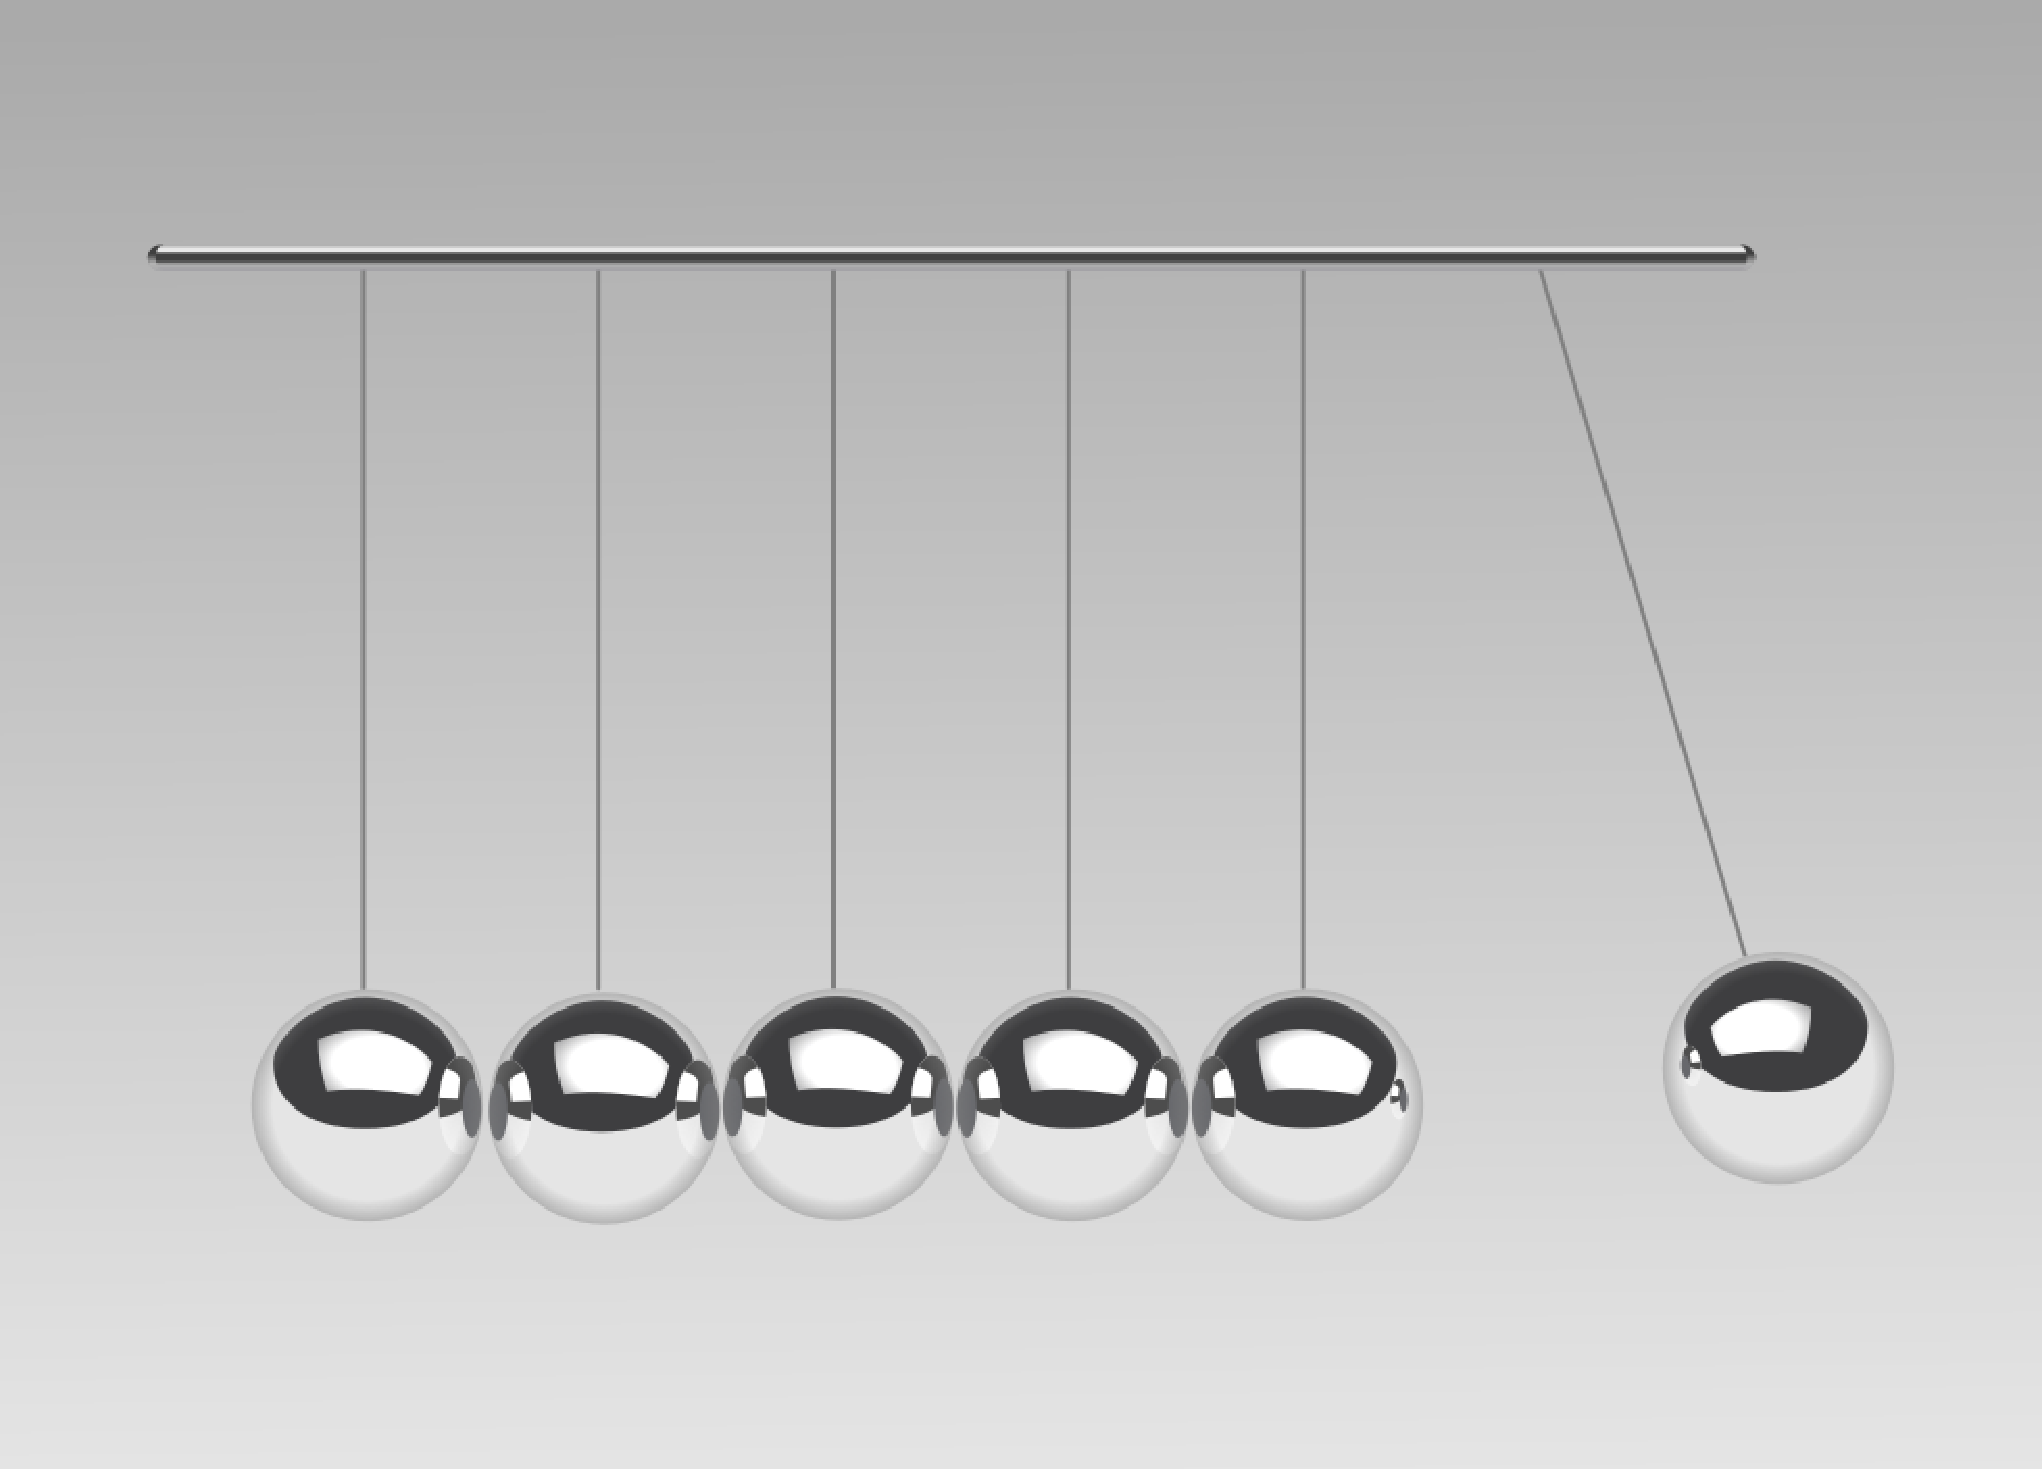
\includegraphics[width=\columnwidth]{newtons_cradle}
  \caption{Possible logo candidate \cite{Andersson2007}}
  \label{fig:newtons_cradle}
\end{figure}


\section{Background}
\label{sec:background}

Problems we want to solve:
\begin{itemize}
\item one
\item another one
\item and a third one
\end{itemize}


\subsection{Exisiting solutions}
\label{sec:exist-sol}

\subsection{New approach}
\label{sec:exist-sol}
Foo
\lstset{language=python}
\begin{lstlisting}[frame=single]  % Start your code-block

from setuptools import setup

setup(name="impactlib",
      version="0.1.0",
      description="Modelica package manager",
      author="Michael Tiller",
      author_email="michael.tiller@gmail.com",
      url="http://www.xogeny.com/",
      scripts=['scripts/impact.py'],
      packages=['impactlib'])
\end{lstlisting}


Search for librararies is done by executed by doing:
\lstset{language=bash}
\begin{lstlisting}[frame=shadowbox]  % Start your code-block

impact.py search <search term>
\end{lstlisting}

\section{Discussion}
\label{sec:discussion}
%TODO

\section{Conclusion}
\label{sec:conclusion}
%TODO

\bibliography{impact}
\end{document}
